%!TeX spellcheck = fr_FR
\documentclass[letterpaper, 12pt]{article}
\usepackage[top = 1.6cm, left = 2cm, right = 2cm ]{geometry}
\usepackage[pdftex]{graphicx}
\usepackage{soulutf8}
\usepackage{amsmath}
\usepackage{tikz}
\usepackage[utf8]{inputenc}
\usepackage{longtable}
\usepackage[T1]{fontenc}
\usepackage{epigraph}
\usepackage{fancyhdr}
\usepackage{float}
\usepackage{subfig}
\usepackage{xcolor}
\usepackage{eurosym}
\usepackage{calc}
\usepackage{multirow} 
%
%
%%%%% Custom commands
%
%
\def\changemargin#1#2{\list{}{\rightmargin#2\leftmargin#1}\item[]}
\let\endchangemargin=\endlist 
%
\newcommand{\newlinealinea}{
~\\ \hspace*{0.5cm}}
%
\newcommand{\alinea}{
\hspace*{0.5cm}}
%
\newcommand{\alinealong}{
\hspace*{1.1cm}}
%
\newcommand{\alignparagraph}{
\hspace*{0.6cm}}
%
\newcommand{\red}[1]{
	\textcolor{red}{#1}}
%
\newcommand{\green}[1]{
	\textcolor{green}{#1}}
%
\newcommand{\point}{$\bullet\ $}
%
\makeatletter
	\newcommand*{\whiten}[1]{\llap{\textcolor{white}{{\the\SOUL@token}}\hspace{#1pt}}}
	\newcommand{\myul}[1]{
		\underline{\smash{#1}}
	}
\makeatother
%
\setlength{\fboxsep}{2pt}
%
\DeclareMathOperator*{\argmax}{\arg\!\max}
%
%
%%%%% Custom text
%
%
\makeatletter
\@addtoreset{section}{part}
\makeatother  
\renewcommand\partname{Partie} 
%
\renewcommand*\sfdefault{phv}
\renewcommand*\rmdefault{ppl}
%
\renewcommand\epigraphflush{flushright}
\renewcommand\epigraphsize{\normalsize}
\setlength\epigraphwidth{0.7\textwidth}
%
\definecolor{titlepagecolor}{cmyk}{0.24,0.92,0.78,0.25}
\definecolor{red}{cmyk}{0, 0.91, 0.91, 0.20}
%
\DeclareFixedFont{\titlefont}{T1}{phv}{\seriesdefault}{n}{0.375in}
%
%
%%%%% Header
%
%
\pagestyle{fancy}
\lhead{Anthony Rouneau}
\rhead{MAB2 Sciences Informatiques}
\cfoot{\thepage}
%
%
%%%%% Title page. The following code is borrowed from: 
%%%%%       http://tex.stackexchange.com/a/86310/10898
%
%
\newcommand\titlepagedecoration{%
\begin{tikzpicture}[remember picture,overlay,shorten >= -10pt]

\coordinate (aux1) at ([yshift=-70pt]current page.north east);
\coordinate (aux2) at ([yshift=-460pt]current page.north east);
\coordinate (aux3) at ([xshift=-6cm]current page.north east);
\coordinate (aux4) at ([yshift=-150pt]current page.north east);

\begin{scope}[titlepagecolor!40,line width=12pt,rounded corners=12pt]
\draw
  (aux1) -- coordinate (a)
  ++(225:5) --
  ++(-45:5.1) coordinate (b);
\draw[shorten <= -10pt]
  (aux3) --
  (a) --
  (aux1);
\draw[opacity=0.6,titlepagecolor,shorten <= -10pt]
  (b) --
  ++(225:2.2) --
  ++(-45:2.2);
\end{scope}
\draw[titlepagecolor,line width=8pt,rounded corners=8pt,shorten <= -10pt]
  (aux4) --
  ++(225:0.8) --
  ++(-45:0.8);
\begin{scope}[titlepagecolor!70,line width=6pt,rounded corners=8pt]
\draw[shorten <= -10pt]
  (aux2) --
  ++(225:3) coordinate[pos=0.45] (c) --
  ++(-45:3.1);
\draw
  (aux2) --
  (c) --
  ++(135:2.5) --
  ++(45:2.5) --
  ++(-45:2.5) coordinate[pos=0.3] (d);   
\draw 
  (d) -- +(45:1);
\end{scope}
\end{tikzpicture}%
}
%
\begin{document}
	\begin{titlepage}
	%
	\noindent
	%
	\newgeometry{bottom = 2cm, top = 2.5cm}
	\begin{center}
		
\includegraphics[scale=1.2]{Images/UMONS}\\
			\vspace*{0.3cm}
		
\includegraphics[scale=0.23]{Images/FS_Logo}\\
			\vspace*{2.5cm}
		%
		\titlefont Image Analysis\\~\\ {\huge Résumé} \par
		%
	\end{center}
	\vspace*{3cm}
	\hfill
	%
	\begin{minipage}{0.18\linewidth}
		\begin{flushright}
			\rule{0.5pt}{75pt}
		\end{flushright}
	\end{minipage}
	%
	\begin{minipage}{0.8\linewidth}
		\begin{flushleft}
			\textsf{\textbf{Résumé réalisé par:}} Anthony Rouneau\\
			\textsf{\textbf{Section:}} 2$^{\text{\`eme}}$ Bloc Master en 
				Sciences Informatiques\\
			\textsf{\textbf{Images:}} Proviennent du cours de M. Mancas.\\
		\end{flushleft}
	\end{minipage}
	%
	\vspace*{\fill}                                                             
	%
	\begin{center}
		Faculté des Sciences $\bullet$ Université de Mons $\bullet$ 
		Place du Parc 20 $\bullet$ B-7000 Mons
	\end{center}
	%
	\titlepagedecoration
	%
\end{titlepage}
%
%
%%%% Tables des matières
%
%
\newgeometry{top = 3cm, left = 2cm, right = 2cm, bottom=2.5cm}
%
\tableofcontents
%
\newpage
%
%
\section{Introduction}
	\subsection{Acquisition d'images}
		\alinea Une image consiste en une matrice de pixels. Il y a trois notions à retenir : 
			\begin{itemize}
				\setlength\itemsep{0cm}
				\item \'Echantillonnage -- Nombre de pixels contenus dans l'image (e.g. 800x600)
				\item Quantization -- Sur combien de bits est encodé chaque dimension du pixel ? (e.g. 8 bits => 255)
				\item Dimension -- Les informations contenues dans chaque pixels : 
				\begin{itemize}
					\setlength\itemsep{0cm}
					\item 2D : niveau de gris
					\item 2.5D : vidéo en niveau de gris
					\item 3D : couleurs
					\item 3.5D (4D) : vidéo couleur
					\item ND : imagerie satellite, nuages de points, ...
				\end{itemize}
			\end{itemize}	
		%
	%
	\subsection{Fréquences}
		\begin{itemize}
			\setlength\itemsep{0cm}
			\item \red{Lumière visible} -- entre 425 et 750 THz, à une longueur d'onde entre 440 et 700nm.
			\item \red{Ultrason} -- entre 1 et 20MHz, utilisé notamment pour les échographies.
			\item \red{Résonance magnétique} -- entre 40 et 50 MHz, analyse le spin des protons dans l'eau (au + d'eau au + de détails).
			\item \red{Terahertz} -- entre 0.2 et 4 THz, utilise deux lasers : un normal et un qui touche un obstacle, puis 
				compare les deux lasers. Si pas de différence, l'objet est plat. Utilisé pour la sécurité, détecter des formes (armes)
				sous les vêtements.
			\item \red{Infrarouge} -- entre 0.7 et 10$\mu$m, nécessite des caméras plus froide que l'environnement, et peu être
				combiné avec une illumination IR.
			\item \red{Rayons-X} -- entre 0.1 et 10 Angström, met en évidence ce que l'IRM ne met pas en évidence (os).
			\item \red{Rayons Gamma} -- entre 0.1 et 0.01 Angström, on fait rencontrer des électrons et des positrons pour 
				libérer de l'énergie et la capter ensuite.
		\end{itemize}
	%
	\subsection{Types d'yeux}
		\alinea Il existe de multiples types d'yeux dans le royaume animal. On peut noter que les "pinholes" ont besoin d'ouvrir
			le trou pour avoir plus de lumière mais qu'au plus ils l'ouvre, au moins ils ont de détails. Quant aux "concaves", 
			ils ne sont pas précis, mais ils sont bons pour suivre des mouvements rapides (cf image page suivante).
			\hl{Contrairement aux caméras, les yeux humains ne reçoivent pas la même quantité de lumière sur toute la surface} de
			la rétine (précis au milieu, moins précis sur les côtés). Et là où les hommes ont des \hl{bâtonnets} (Rod, vision noir et blanc
			pour la nuit) et des \hl{cônes} (vision couleur en journée), une caméra n'a que des pixels, généralement en couleurs.
		%
		\begin{center}
			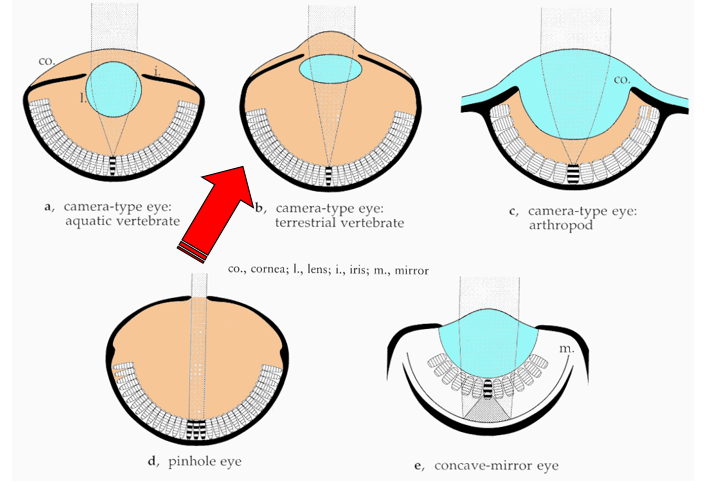
\includegraphics[width=5.5in]{Images/eyes}
		\end{center}
	%
	\subsection{Types de CCD}
		\alinea Les caméra modernes sont composées de 3 éléments principaux : l'\hl{iris} (lumière), la \hl{lentille} (focus) et 
			les \hl{CCD} (Charged Couple Device, donnent les composantes des pixels). \hl{Toute la surface est éclairée de la même
			manière}, ce qui permet d'avoir une image aussi nette au centre que sur les côtés. Un CCD contient une quantité de 
			lumière (monochromatique).\\
		%
		~\\
		%
		\alinea Plusieurs architectures ont vu le jour. La première (ci-dessous à gauche) avait une bonne résolution, mais 
			provoquait des "\hl{smears}" (ci-dessous, à gauche) dû aux phases d'\hl{exposition et de lecture} qui se produisaient 
			en même temps. On devait donc avoir recours à des \hl{fermetures mécaniques} pour stopper l'exposition (ralenti le temps
			entre deux prises...).
		\begin{center}
			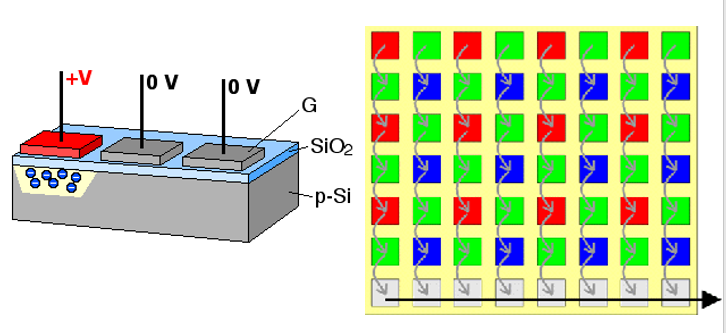
\includegraphics[width=4in]{Images/ccd1} 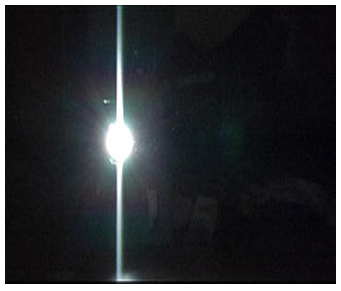
\includegraphics[width=2in]{Images/smear}
		\end{center}
		%
		\pagebreak
		%
		\alinea C'est pourquoi des capteurs plus intelligents ont été développés, proposant une surface d'exposition séparée de la
			surface de lecture afin d'\hl{éviter la sur-exposition}.
		\begin{center}
			\begin{minipage}{0.33\textwidth}
				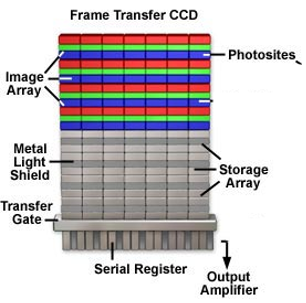
\includegraphics[width=2.5in]{Images/ccd2} \hfill 
			\end{minipage}
			\begin{minipage}{0.33\textwidth}
				\begin{flushleft}
				~\\
				$\leftarrow$ Très rapide, haute résolution et capture de toute la lumière, mais un peu de smearing quand même.
				\end{flushleft}
				\begin{flushright}
				 Rapide, peu de smearing $\rightarrow$
				 faible résolution car espace coupé par les cellules de stockage.	
				 \end{flushright} 
			\end{minipage}		
			\begin{minipage}{0.32\textwidth}
				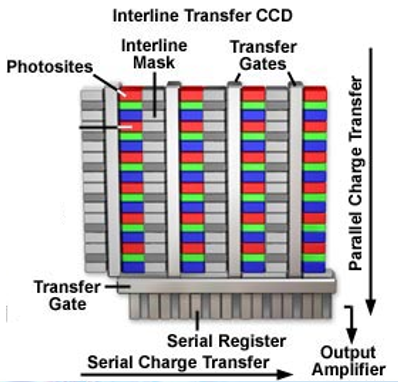
\includegraphics[width=2.75in]{Images/ccd3}
			\end{minipage}
		\end{center}
		%
		\alinea Il y a eu aussi les lignes de CCD (fax, scanner) qui ont besoin de se déplacer sur l'objet pour prendre la photo complète.
		\begin{center}
			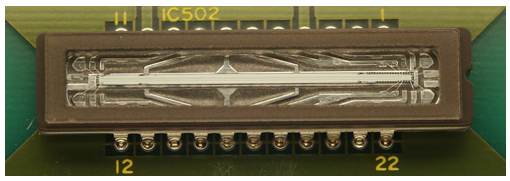
\includegraphics[width=2in]{Images/ccd4}
		\end{center}
		%
		\alinea Enfin, les avancées technologiques on permis l'arrivée du Super-CCD et du CMOS. Le \hl{Super-CCD} (à gauche) est
			intéressant de part la forme des cellules qui permette de couvrir \hl{90\% de la surface exposée}, tout en gardant les 
			lignes permettant la \hl{sauvegarde directe} des pixels. On utilisait des lentilles pour concentrer la lumière sur les cellules. 
			Les \hl{CMOS} (à droite) quant à eux sont plus simples à construire, et sont donc \hl{moins chers}, ont une sauvegarde 
			\hl{plus rapide} (RAM), mais une résolution moins grande (\hl{30\% de couverture}).
		\begin{center}
			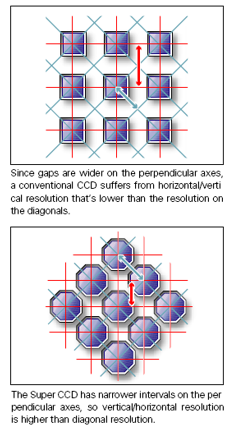
\includegraphics[width=1.5in]{Images/ccd5} \hfill 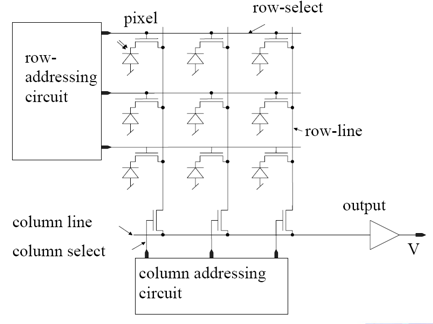
\includegraphics[width=3.5in]{Images/cmos}
		\end{center}
		%
	%
	\subsection{Camera couleur}
		\alinea Deux stratégies existent : un \hl{prisme} qui vient diviser la lumière en 3 composantes RGB, chacune exposée sur une 
			plaque CCD différente, ou \hl{bayer} permettant une interpolation bilinéaire.
		%
		\begin{center}
			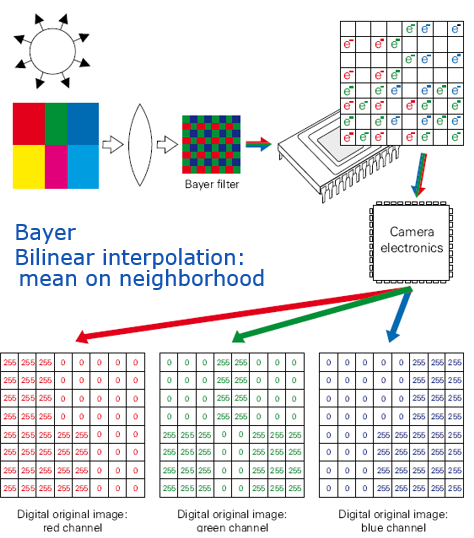
\includegraphics[width=3.5in]{Images/bayer}
		\end{center}
		%
	%
%
\section{Pixels}
	\alinea Les pixels d'une images sont caractérisés par leur \hl{position dans l'espace} et par leur \hl{valeur}
		(Pixel 3D = Voxel).
	%
	\subsection{Distance}
		\alinea Il existe plusieurs mesures de distances :
		$$ d_1(p, q) = |x_p - x_q| + |y_p - y_q| $$
		$$ d_2(p, q) = \sqrt{(x_p - x_q)^2 + (y_p - y_q)^2} $$
		$$ d_{inf}(p, q) = \max{(|x_p - x_q|, |y_p - y_q|)} $$
		$$ \forall p, q : d_{inf}(p, q) <= d_2(p, q) <= d_1(p, q) $$
		%
	%
	\subsection{Voisinage}
		\alinea Le \hl{voisinage} d'un pixel est défini comme suit :
			$$ V_k(p) = {q: 0 < d(p, q) <= k} $$
		%
		\alinea On peut parler de connexion entre pixels. Il y a plusieurs manière de les \hl{connecter} :
			\begin{center}
				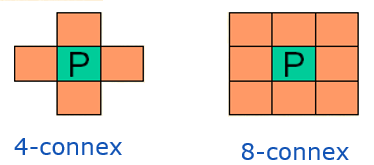
\includegraphics[width=3in]{Images/connex}
			\end{center}
		%
	%
	\subsection{Représentation des couleurs}
		\subsubsection{Systèmes additifs/soustractifs}
			\paragraph{RGB (additif)}~\\~\\
				\alinea Combinaison de rouge, vert et bleu. Chaque valeur étant encodé sur 8 bits.
			%
			\paragraph{CYMK (soustractif)} ~\\~\\
				\alinea Des valeurs de \hl{cyan, jaune et magenta} sont \hl{retirées} à la lumière blanche pour former une couleur.
					Une \hl{clé (K) de densité} de noir a été ajouté parce que la combinaison CYM n'était pas parfaite.
			%
		%
		\subsubsection{Séparation luminance/chrominance}
			\paragraph{HSV (HSI)}~\\~\\
				\alinea Trois valeurs : \hl{Hue}, en degrés (entre 0 et 360$^o$) représentant la longueur d'onde de la couleur,
					\hl{Saturation}, représentant l'intensité de la couleur (pureté) et \hl{Value}, représentant l'intensité de
					lumière dans la couleur. Les systèmes YUV et YCbCr utilisent un, système similaire.
				%
			\paragraph{LAB}~\\~\\
				\alinea Trois valeurs : \hl{L} pour l'intensité de lumière, \hl{A} pour un mélange de vert et de magenta, et 
					\hl{B} pour un mélange de bleu et de jaune.
				%
			%
			\paragraph{Opponent color system}~\\~\\
				\alinea Système utilisé par les hommes. La luminance est associée aux bâtonnets (rods) et la chromance aux cônes.
				%
			%
		%
	%
	\subsection{Amélioration basique d'image}
		\subsubsection{Amélioration d'histogramme}
			\alinea On peut améliorer une image en modifiant son \hl{histogramme}. L'histogramme s'obtient en comptant le nombre
				de pixels par valeur de pixel (par ex. combien de pixels en niveau de gris ont 30 comme valeur ?). 
				L'idée est ensuite de répartir les valeurs pour améliorer la distribution des nuances de gris.
			%
			\paragraph{\'Egalisation d'histogramme}~\\~\\
				\alinea L'idée ici est de \hl{répartir les valeurs sur tout l'histogramme} pour obtenir un contraste plus élevé.
					\begin{center}
						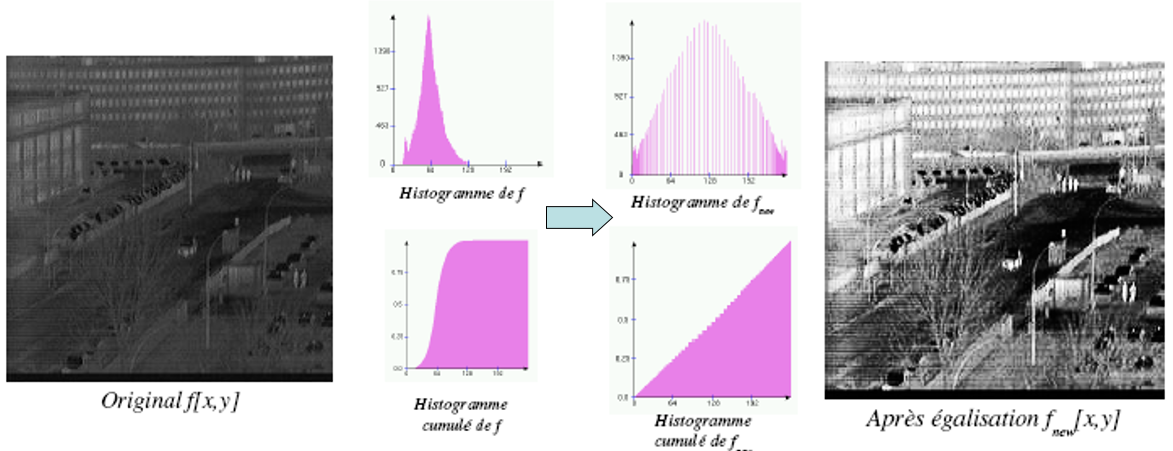
\includegraphics[width=6in]{Images/histo1}
					\end{center}
					\begin{center}
						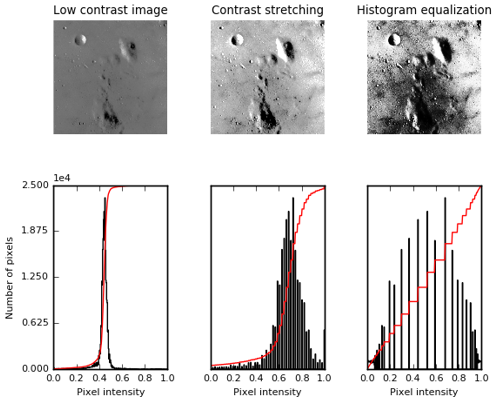
\includegraphics[width=3in]{Images/histo2}
					\end{center}
				%
			%
			\paragraph{Dilatation des zones sombres/lumineuses}~\\~\\
				\alinea On peut rendre une image plus claire, plus sombre, ou en tout cas améliorer son contraste en ne \hl{modifiant
					qu'une partie de l'histogramme}.
				%
				\begin{center}
					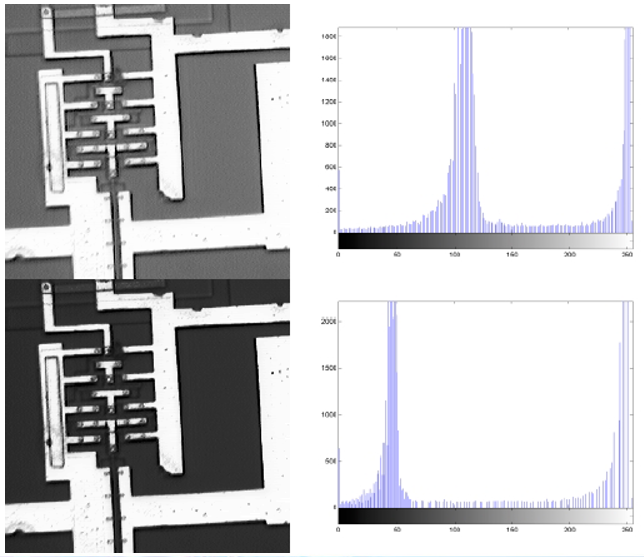
\includegraphics[width=3in]{Images/histo3} \hfill 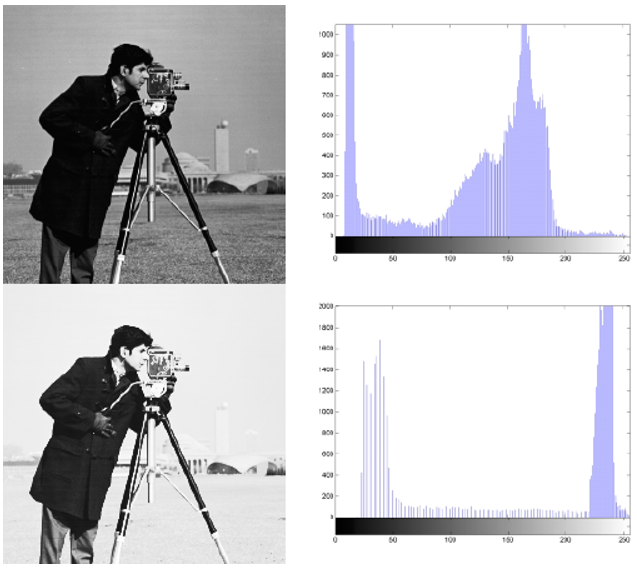
\includegraphics[width=3in]{Images/histo4}
				\end{center}
				%
			%
		%
		\subsubsection{Fausses couleurs}
			\alinea L'être humain est plus sensible aux nuances de couleurs qu'aux nuances de gris ! Ceci s'explique par le fait
				que les couleurs sont gérées par les cônes, qui influent sur les détails et la "haute résolution" de la vue.
				C'est pourquoi des images grises sont parfois colorisées pour mettre en évidence les détails.
				\begin{center}
					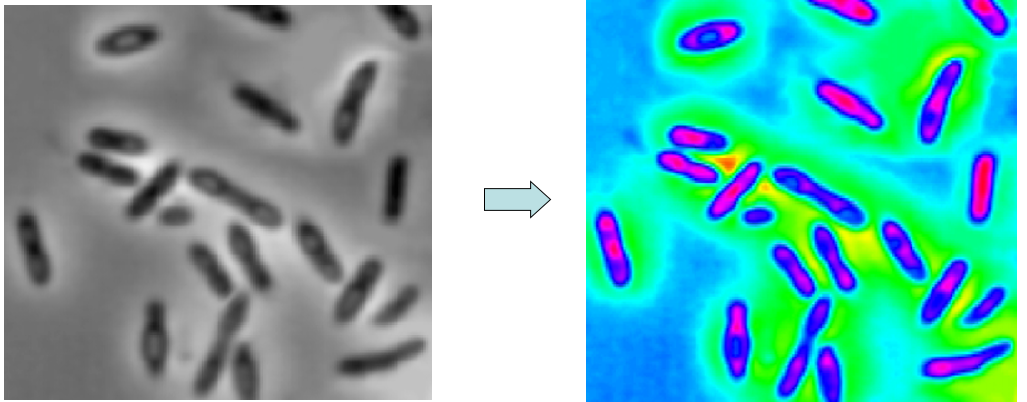
\includegraphics[width=2.5in]{Images/false}
				\end{center}
			%
		%
	%
%
\pagebreak
%
\section{Filtrage spatial}
	\alinea La notion de fréquence dans une image s'applique aux variations de valeur dans les zones de l'images.
		Les \hl{basses fréquences} représentent des zones homogènes, à faible variations, tandis que les \hl{hautes fréquences}
		représentes des bords, des coins, des textures, etc...
	%
	\subsection{Corrélation}
		\alinea Ce qu'on appelle en générale une convolution en analyse d'image est en réalité bien souvent une \hl{corrélation}.
			\begin{center}
				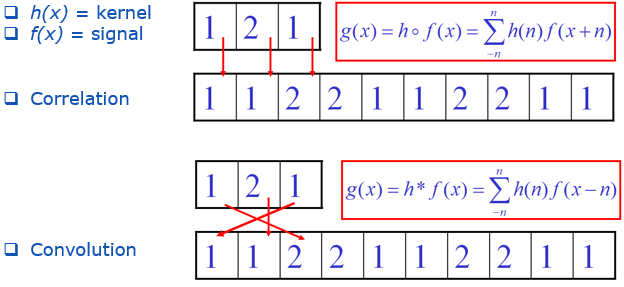
\includegraphics[width=3.75in]{Images/correlation}
			\end{center}
			\begin{center}
				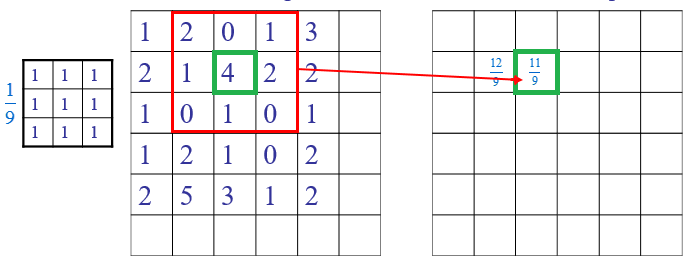
\includegraphics[width=4.5in]{Images/correlation2}
			\end{center}
		%
		\alinea \'Etant donné qu'on a \hl{besoin d'aller au delà des bords} afin de calculer la nouvelle valeur de ces bords, plusieurs
			techniques existent: copier les bords existant, utiliser des 0, utiliser des valeurs miroir aux bords ou encore
			utiliser une technique d'indexation circulaire (par un modulo).
		%
		\subsubsection{Passe-bas}
			\alinea Plusieurs kernels passe-bas existent, comme par exemple : \\
				$$\frac{1}{9} \cdot \begin{bmatrix} 1&1&1\\ 1&1&1\\1&1&1\\ \end{bmatrix}\text{,} 
				\frac{1}{10} \cdot \begin{bmatrix} 1&1&1\\ 1&2&1\\1&1&1\\ \end{bmatrix}\text{, ou encore}
				\frac{1}{16} \cdot \begin{bmatrix} 1&2&1\\ 2&4&2\\1&2&1\\ \end{bmatrix}\text{.}$$\\
				On peut remarquer que la "connexion" entre pixels est considérée différemment dans chacun de ces kernels.
				Ces filtres rende l'image "\hl{floue}".
			%
		%
		\subsubsection{Passe-haut}
			\alinea Exemples de kernel passe-haut du premier ordre : \\
			$$\begin{bmatrix} -1&-1&-1\\ -1&+8&-1\\-1&-1&-1\\ \end{bmatrix} \text{(4-connex),} 
			\begin{bmatrix} 0&-1&0\\ -1&+4&-1\\0&-1&0\\ \end{bmatrix} \text{(8-connex)}$$\\ ou encore un filtre Laplacien du
			\hl{second degré qui permet d'isoler les contours} (le cerveau humain utilise une sorte de filtre du second degré pour
			isoler les bords). Comme les hautes fréquences représente des bords, il peut être 
			intéressant de \hl{filtrer dans une	direction}. Voici 4 exemples de filtres directionnels (certaines cellules du cerveau
			fonctionnent comme des filtres directionnels).
			\begin{center}
				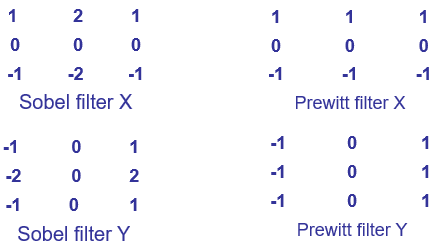
\includegraphics[width=3in]{Images/directional} \hfill 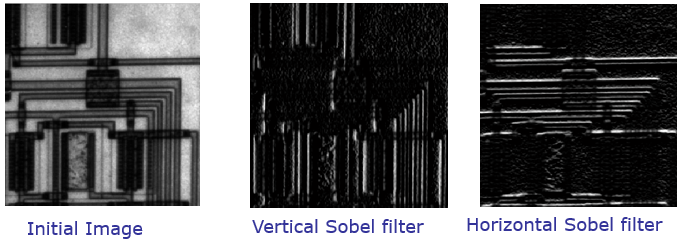
\includegraphics[width=3.75in]{Images/directional2}
			\end{center}
		%
	%
	\subsection{Filtres de rang}
		\alinea Le principe ici est de choisir un élément selon sa position ou sa valeur dans le kernel. Voici par exemple
			un filtre médian, qui donne un résultat \hl{moins flou qu'un passe bas} (car on utilise des valeurs existant déjà).
			\begin{center}
				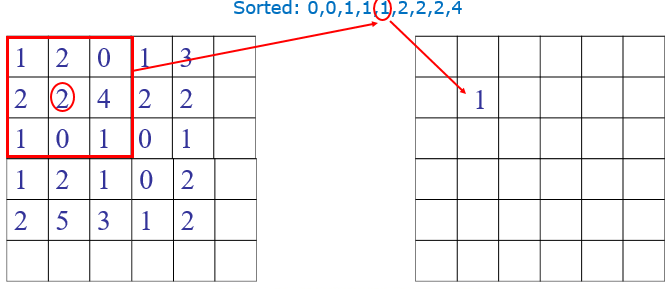
\includegraphics[width=4in]{Images/rank}
			\end{center}
		%
		\alinea D'autres opérations que "médian" existent, comme max, min, range (max-min), random, etc...
		%
	%
	\subsection{Filtres morphologiques}
		\alinea Ces filtres utilisent une forme géométrique (structuring element, ou S) pour s'appliquer sur l'image.
		%
		\subsubsection{\'Erosion}
			\alinea Le principe de ce filtre est de \hl{supprimer (remplacer par des 0) les éléments plus petits} que le 
				structuring element.
				Lorsque S est placé  entre des 0 et des 1, on efface les 1 en les remplaçant par des 0. Les objets plus petits que 
				2 fois la taille de S seront supprimés. Faire une érosion avec S de taille N est similaire à faire N érosions
				avec S de taille 1. \hl{(Dilate le noir -- background)}
			%	
			\begin{center}
				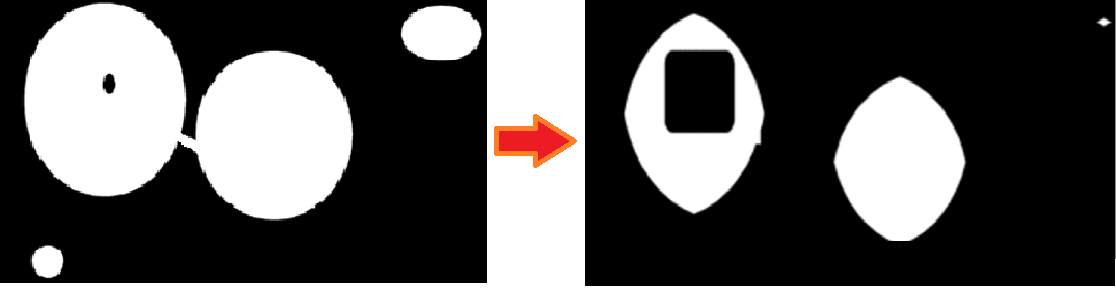
\includegraphics[width=3.5in]{Images/erosion}
			\end{center}
			%
			\begin{minipage}{0.33\textwidth}
				\alinea Si on l'applique au niveau de gris plutôt que sur une image binaire, les éléments prennent la \hl{valeur minimale}
					dans le champ de S. (Dans l'exemple, S=B et à comme taille trois bâtonnets du graphe).
			\end{minipage} \hfill
			\begin{minipage}{0.66\textwidth}
				\begin{center}
					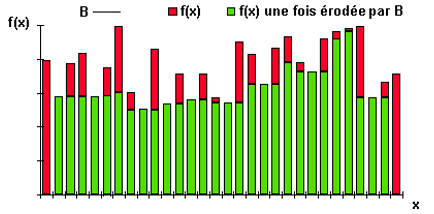
\includegraphics[width=3.95in]{Images/erosion2}
				\end{center}
			\end{minipage}
			%
		%
		\subsubsection{Dilatation}
			\alinea Le principe de ce filtre (dilation en anglais) est de \hl{rajouter (remplacer par des 1) les éléments plus petit} 
				que le structuring element.	Lorsque S est placé  entre des 0 et des 1, on efface les 1 en les remplaçant par des 0. 
				Les objets plus petits que 2 fois la taille de S seront connectés. \hl{(Dilate le blanc -- foreground)}
			%	
			\begin{center}
				
\includegraphics[width=3.5in]{Images/dilation}
			\end{center}
			%
			\begin{minipage}{0.33\textwidth}
				\alinea Si on l'applique au niveau de gris plutôt que sur une image binaire, les éléments prennent la \hl{valeur maximale}
					dans le champ de S. (Dans l'exemple, S=B et à comme taille trois bâtonnets du graphe).
			\end{minipage} \hfill
			\begin{minipage}{0.66\textwidth}
				\begin{center}
					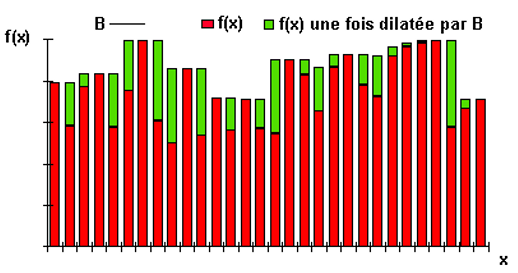
\includegraphics[width=3.95in]{Images/dilation2}
				\end{center}
			\end{minipage}
			%
		%
		\subsubsection{Ouverture}
			\alinea Le principe de ce filtre est de \hl{faire suivre une érosion d'une dilatation}. Ça a pour effet d'ouvrir (supprimer) 
				les petits (selon la taille de S) espaces blancs uniquement (les grandes formes sont plus ou moins conservées).
			%	
			\begin{center}
				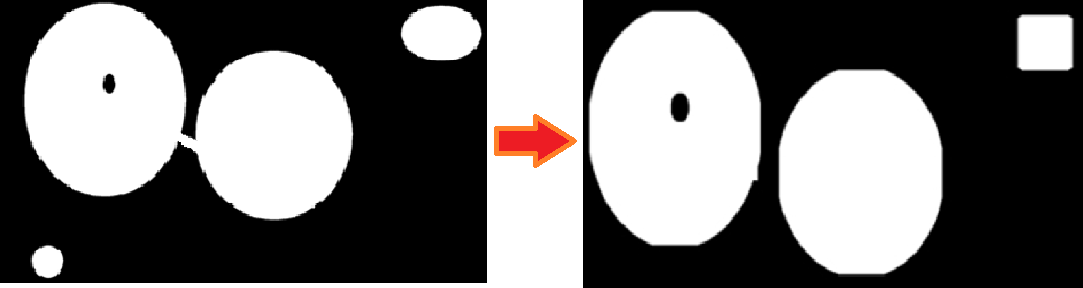
\includegraphics[width=3.5in]{Images/opening}
			\end{center}
			%
		%
		\subsubsection{Fermeture}
			\alinea Le principe de ce filtre est de \hl{faire suivre une dilatation d'une érosion}. Ça a pour effet de fermer 
				(remplacer par des 1) les petits (selon la taille de S) espaces noir uniquement (les grandes formes sont plus ou 
				moins conservées).
			%	
			\begin{center}
				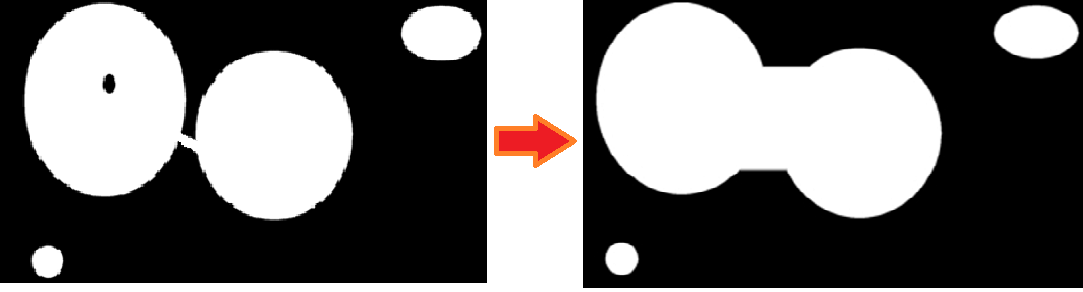
\includegraphics[width=3.5in]{Images/closing}
			\end{center}
			%
		%
		\subsubsection{Skeletonnization}
			\alinea Fait apparaître une sorte de \hl{squelette}. C'est une érosion en série jusqu'à ce qu'il ne reste que 1 pixel.
			\begin{center}
				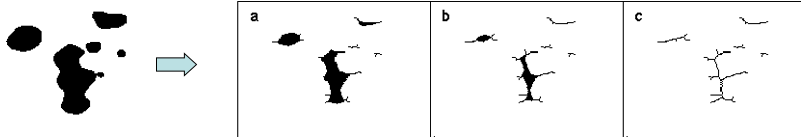
\includegraphics[width=5in]{Images/skeleton}
			\end{center}
			%
		%
	%
%
\section{Transformées d'image}
	\alinea Comme on peut parler de fréquences dans une image, on peut également décomposer ces fréquences et appliquer des opérations
		sur elles.
	%
	\subsection{Transformée de Fourier discrète (DFT)}
		\alinea Le principe de cette transformée et de retrouver les \hl{composantes fréquentielles} de l'image.
		%
		\begin{center}
			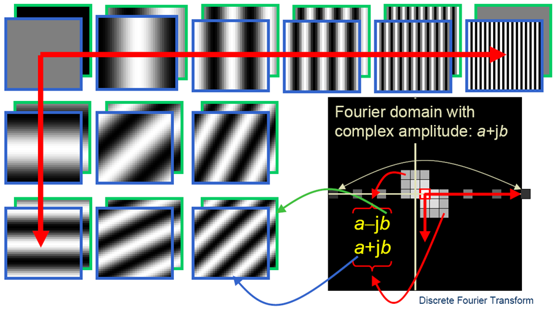
\includegraphics[width=3in]{Images/dft}
		\end{center}
		%
		\subsubsection{Amplitude}
			\alinea Grâce à l'amplitude, on peut voir dans quelles \hl{zones de fréquences il y a beaucoup d'énergie}.
			%
			\begin{center}
				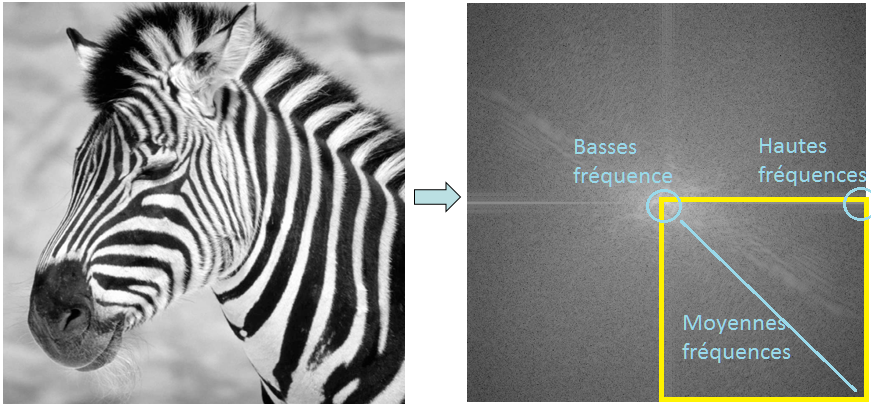
\includegraphics[width=4.75in]{Images/dft2}
				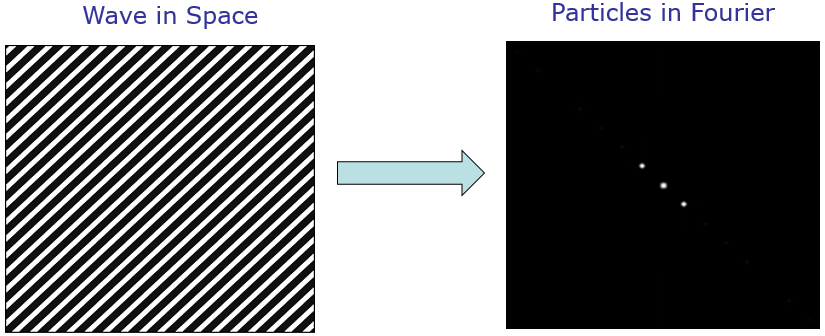
\includegraphics[width=3.5in]{Images/dft3}
				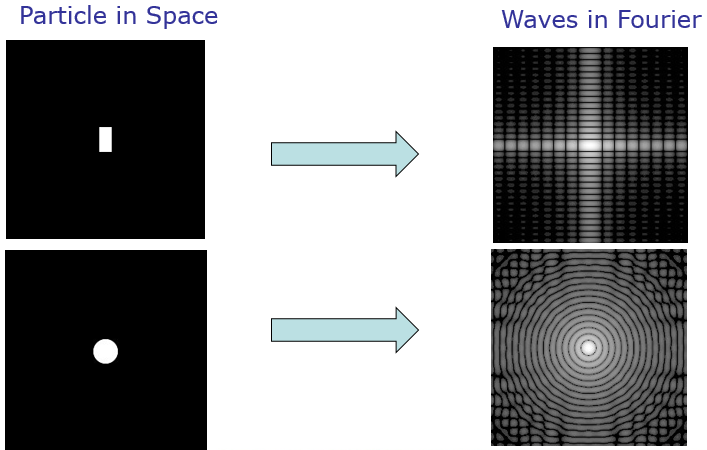
\includegraphics[width=3.5in]{Images/dft4}
			\end{center}
			%
		%
		\subsubsection{Phase}
			\alinea Les phases représente le \hl{décalage par rapport à l'origine de chaque fréquence}. Elles sont importantes au niveau
				de la perception de l'image				
			%
			\begin{center}
				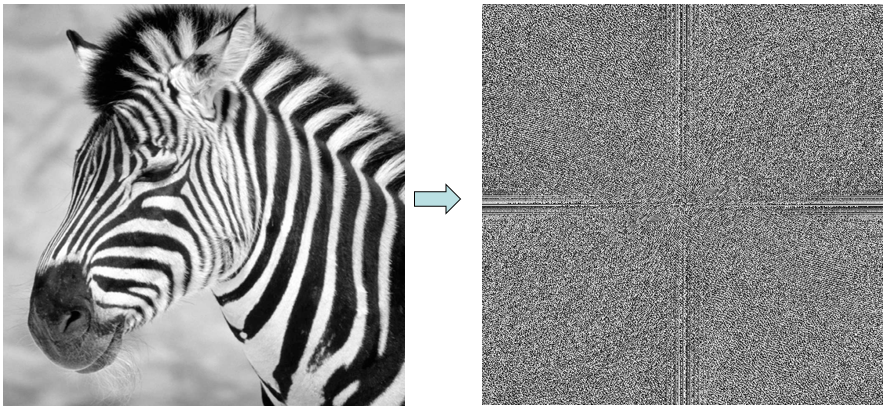
\includegraphics[width=3in]{Images/dft_phase}
				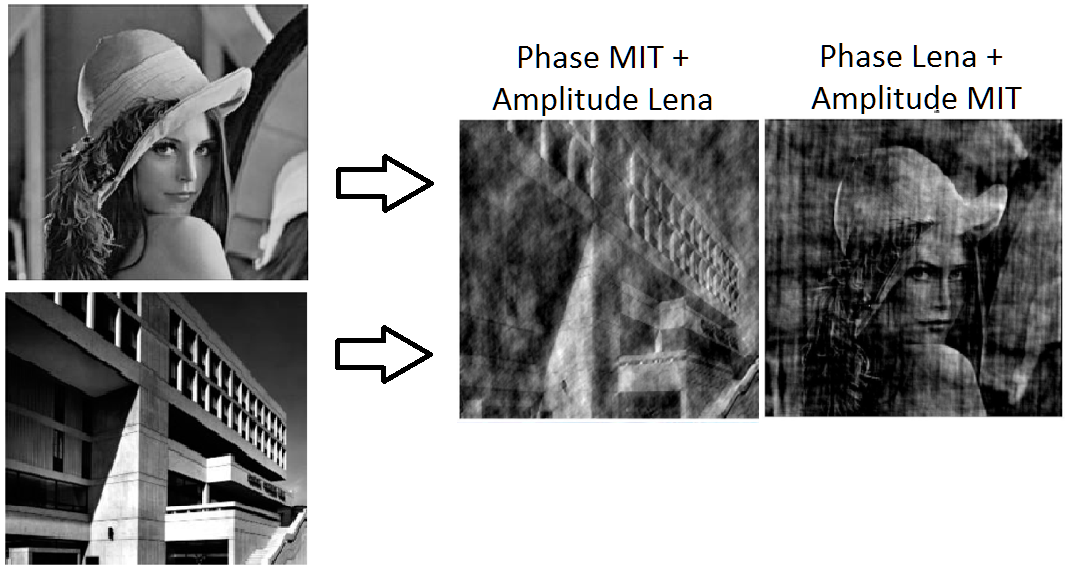
\includegraphics[width=5.5in]{Images/dft_phase2}
				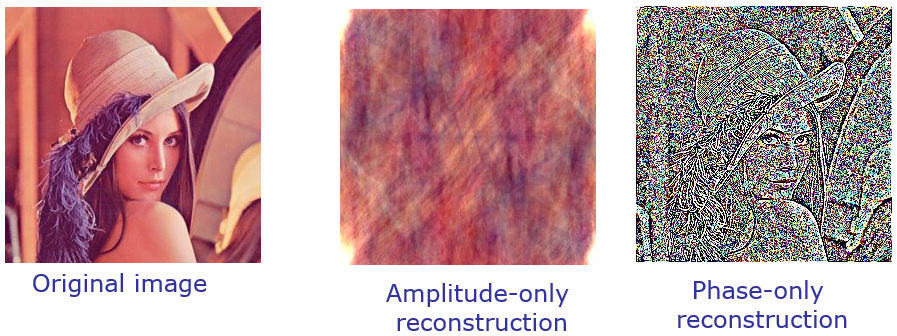
\includegraphics[width=5.5in]{Images/dft_phase3}
			\end{center}
			%
		%
		\subsubsection{Filtrage}
			\alinea On peut utiliser la FFT/DFT pour filtrer une image. En effet, on peut \hl{sélectionner des zones de fréquences},
				et mettre tout le reste à zéro. Ainsi, pour un passe bas, il suffit de garder le centre de l'amplitude de l'FFT.
				\hl{C'est plus rapide pour les grandes images} que d'appliquer des filtres à kernel sur tous les pixels.
			%
			\begin{center}
				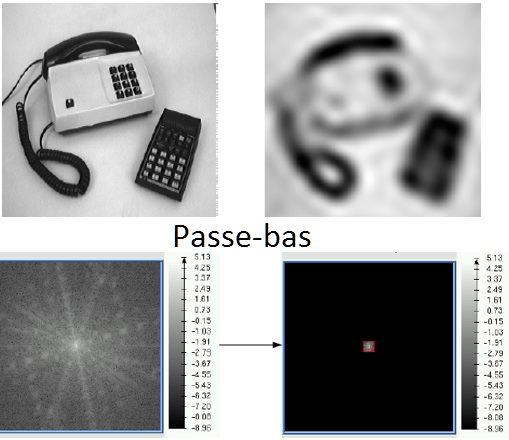
\includegraphics[width=2.75in]{Images/dft_filter1} \hfill 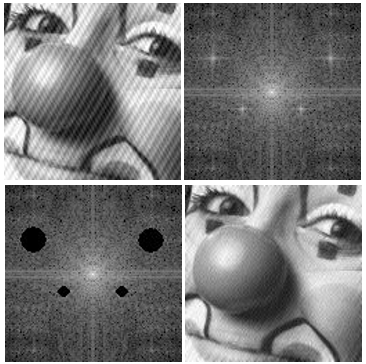
\includegraphics[width=2.33in]{Images/dft_filter3}
				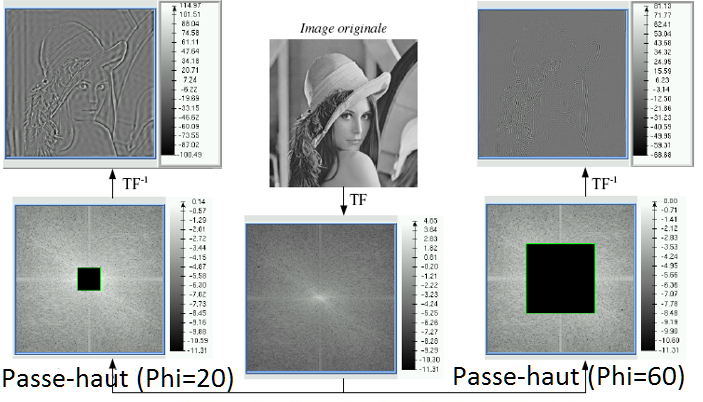
\includegraphics[width=5.25in]{Images/dft_filter2}
			\end{center}
			%
		%
	%
	\subsection{Transformée Radon}
		\alinea Projection de l'\hl{intensité de l'image selon de multiples angles}. Ça revient à prendre des lignes de la DFT selon pleins
			d'angles différents. Lorsqu'on applique cette transformée sur une image dont les bords (im. binaires) ont été mis en évidence, 
			on appelle ça la \red{\hl{Transformée de Hough}}. 
		%
		\begin{center}
			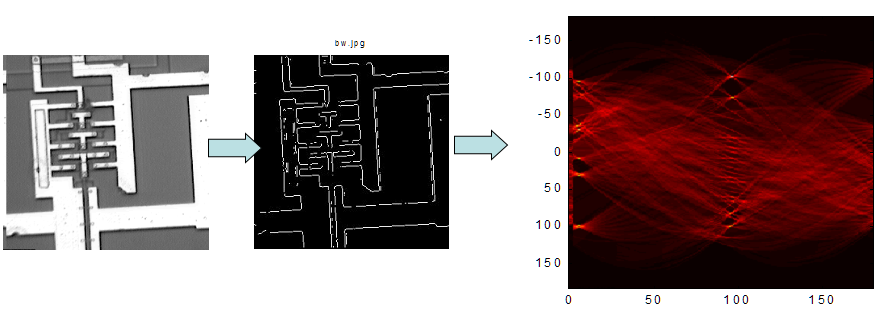
\includegraphics[width=5.5in]{Images/hough}
		\end{center}
		%
	%
	\subsection{Transformée cosine discrète (DCT)}
		\alinea Similaire à une DFT, mais où il n'y a que des nombres réels, et qui permet d'\hl{approximer les lignes avec moins de 
			coefficients dans les calculs}. Moins bon que la DFT pour le reste.
		%
	%
	\subsection{Transformée spatiale (PCA)}
		\alinea Le but est de \hl{rendre les données non-corrélées} et de ne garder que les informations importantes.
			Effectue une \hl{rotation des données }en utilisant des axes rendant les données non-corrélées.
			Ce qui la rend \hl{différente de la DFT}, c'est qu'elle se base sur les données et non sur les cos/sin.
		%
	%
	\subsection{Transformées spatiale/fréquence}
		\alinea Le problème avec \hl{Fourier, c'est qu'on perd l'information spatiale} (où se trouve l'élément dont la fréquence est ...).
			On va donc chercher à pouvoir \hl{exploiter à la fois les fréquences, et les données spatiales}.
		%
		\subsubsection{Filtre de Gabor}
			\alinea Le principe est d'appliquer une\hl{ DFT sur une fenêtre gaussienne} 
				(afin d'analyser les fréquence d'une partie de l'image).
				\begin{center}
					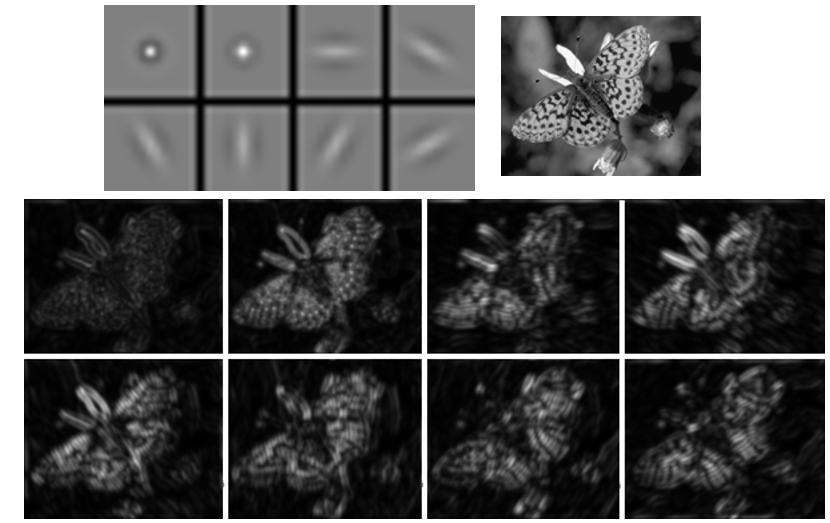
\includegraphics[width=5.5in]{Images/gabor}
				\end{center}
			%
		%
		\subsubsection{Ondines discrètes (Wavelet)}
			\alinea Le principe est de \hl{décomposer l'image en plusieurs composantes filtrées}. La reconstruction de ces composantes
				redonne (avec une petite erreur) l'image de base. Pour décomposer l'image, on a besoin de formes d'ondines (wavelets).
				Chaque wavelet donnera sa composante. 
			%
			\begin{center}
				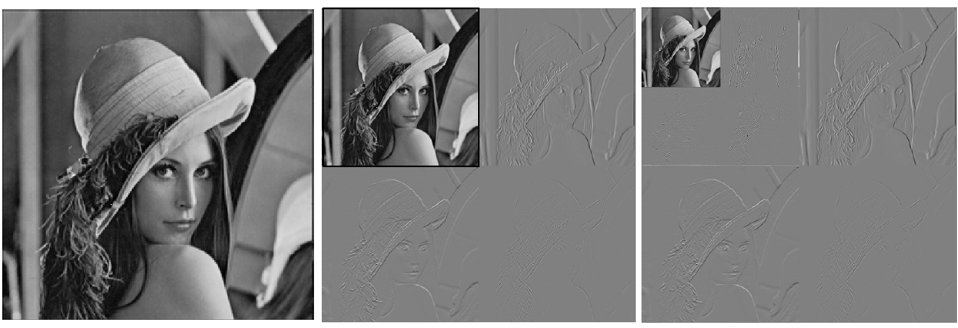
\includegraphics[width=6in]{Images/wavelets2}
			\end{center}
			%
			\alinea En pratique on utilise des banques de données de wavelets qui permettront une reconstruction.			
			%
			\begin{center}
				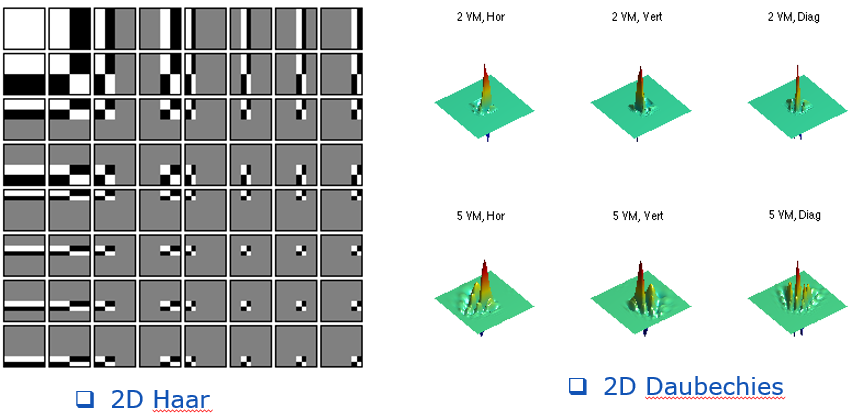
\includegraphics[width=4.75in]{Images/wavelets}
			\end{center}
			%
		%
	%
%
\section{Comparaison d'images}
	\alinea Il est difficile de comparer deux images qui n'ont pas été pris au même moment, par le même appareil et selon des
		points de vue différents. On va alors chercher à \hl{trouver une transformée géométrique permettant d'aligner les pixels}
		du mieux possible afin de pouvoir dire si les deux images représentent le même objet, la même personne, ...\\
		On est alors confrontés à \hl{4 problèmes} :
		\begin{itemize}
			\setlength\itemsep{0cm}
			\item Extraire des repères communs.
			\item \'Etablir une mesure de similarité selon les repères détectés.
			\item Trouver la transformée géométrique.
			\item Optimiser le processus.
		\end{itemize}
	%
	\subsection{Extraire des repères}
		\alinea Il y a plusieurs manières de procéder : 
		\begin{itemize}
			\setlength\itemsep{0cm}
			\item \red{Repères géométriques} : pas utile si l'image a été pris d'un point de vue différent.
			\item \red{Repères d'intensité} : on note les \hl{changements d'intensités dans les couleurs/nuances} ou autres mesures.
			\item \red{Repères pré-établis} : on peut facilement retrouver des repères pré-établi ayant une particularité (couleur vive,
				forme particulière, ...)
		\end{itemize}
		%
	%
	\subsection{Mesure de similarité}
		\alinea Selon une transformée $T$, on estime si les deux images sont équivalentes, à $T$ près grâce à un ensemble 
			de repères (features) $K$:
		$$ S(T) = \sum\limits_{k \ in K} \Vert T(x_k) - y_k \Vert^2 $$
		Dans tous les cas, on compares les deux images selon les repères qui ont été choisis au préalable.
	%
	\subsection{Transformée géométrique}
		\subsubsection{Transformée rigide}
			\alinea Ce type de transformée conserve les distances et les angles. En appliquant une transformée de ce type, on 
				effectue une rotation et/ou une mise à l'échelle des axes et/ou une translation de l'image 
				(\hl{zoom / rotation / translation}).\\
			%
			~\\
			%
			\alinea Pour rester performant au niveau calcul (on évite les additions), 
				on passe par une représentation homogène des coordonnées.
				Dans l'exemple suivant, $(S_x,\ S_y)$ sont des facteurs de redimensionnement, $(\Delta x,\ \Delta y)$ sont
				les coordonnées de translation, et $\theta$ est l'angle de rotation. 
				(2D: 5 paramètres, 3D: 9 paramètres car 3 angles de rotation)
			%
			\begin{center}
				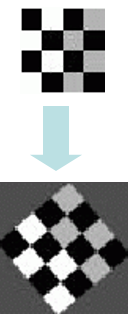
\includegraphics[width=0.66in]{Images/rigid} \hfill 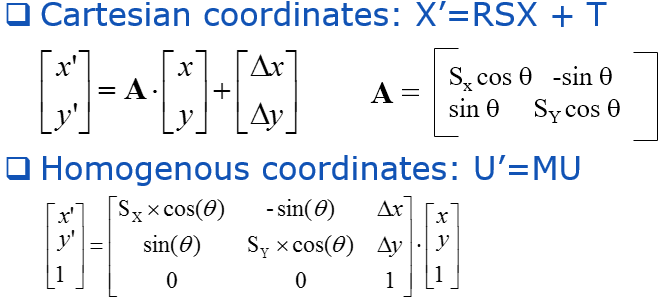
\includegraphics[width=3.75in]{Images/homogenous}
			\end{center}
			%
		%
		\subsubsection{Transformée affine}
			\alinea Ce type de transformée préserve le parallélisme coté à coté, mais ne préserve pas les angles. 
				Dans l'exemple suivant on a $(\Delta x,\ \Delta y)$ qui sont les coordonnées de translation et les
				$a$ qui représentent les changement d'angle (2D: 6paramètres, 3D: 12 paramètres).
			%
			\begin{center}
				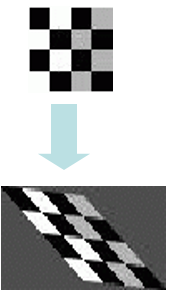
\includegraphics[width=0.6in]{Images/affine} \hfill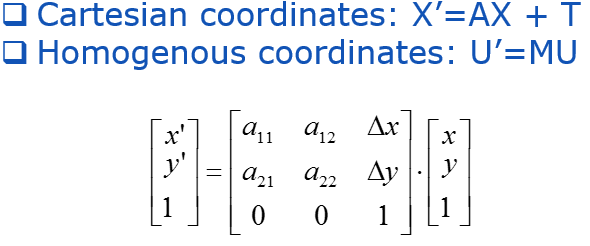
\includegraphics[width=2.75in]{Images/homogenous_affine}
			\end{center}
			%
		%
		\subsubsection{Transformée par projection}
			\begin{minipage}{0.75\textwidth}
				\alinea Ce type de transformée préserve le fait que les lignes soient droites (2D: 9 paramètres, 3D: 16 paramètres).
			\end{minipage} \hfill
			\begin{minipage}{0.24\textwidth}
				\begin{center}
					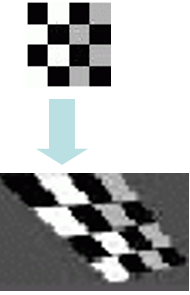
\includegraphics[width=0.6in]{Images/projective}
				\end{center}
			\end{minipage}
			%
		%
		\subsubsection{Transformée incurvée}
			\begin{minipage}{0.75\textwidth}
				\alinea Ce type de transformée ne préserve rien, très difficile à utiliser en pratique...
			\end{minipage} \hfill
			\begin{minipage}{0.24\textwidth}
				\begin{center}
					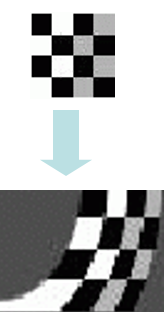
\includegraphics[width=0.6in]{Images/curved}
				\end{center}
			\end{minipage}
			%
		%
	%
	\subsection{Optimisation}
		\alinea On voudrait maintenant trouver une méthode performante qui permettent de trouver automatiquement
			la bonne transformée pour maximiser la similarité entre deux images. Il existe plusieurs méthodes : 
			\begin{itemize}
				\setlength\itemsep{0cm}
				\item Sans calcul de gradients (OK pour les transformées rigides) :
				\begin{itemize}
					\setlength\itemsep{0cm}
					\item Simplexe / Powell -- sensible à l'initialisation des données.
					\item Algorithmes génétiques.
				\end{itemize}
				\item Avec calcul de gradients (on calcule des pentes, et on le fait tant que la pente monte $\Rightarrow$ 
					risque de maxima local):
				\begin{itemize}
					\setlength\itemsep{0cm}
					\item 1$^{\text{er}}$ ordre / 2$^{\text{ème}}$ ordre.
					\item Levenberg-Marquardt -- mélange 1$^{\text{er}}$  et 2$^{\text{ème}}$ ordre.
					\item Gradient conjugué -- utilise le gradient et le gradient précédent.
				\end{itemize}
			\end{itemize}
		%
		\alinea Pour éviter les maxima locaux, on fait souvent appel à une analyse multi-résolution, depuis la résolution
			la plus basse jusqu'à la résolution la plus élevée.
			\begin{center}
				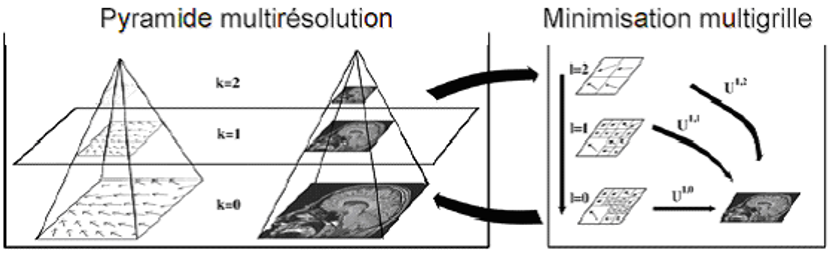
\includegraphics[width=5in]{Images/multi-resolution}
			\end{center}
		%
	%
%
\section{Segmentation}
	\alinea \red{Segmenter} une image c'est prendre des \hl{informations haut niveau} à partir de pixels (bas niveau).
	%
	\subsection{Critères de segmentation}
		\subsubsection{Simples attributs d'image}
			\alinea Les attributs les plus simples d'une image sont les \hl{valeurs des pixels}. \`A partir de ces valeurs,
				on va chercher des inhomogénéités dans l'image, telles que des bords, des différences de couleurs, etc...
				Le problème est que \hl{détecter les bords est une pratique subjective} et dépend de ce que l'on veut 
				détecter exactement. L'exemple suivant montre différentes détections de bords utilisant chacune un seuil de 
				détection différent.
			%
			\begin{center}
				\includegraphics[width=4in]{Images/edges}
			\end{center}
			%
			\alinea La technique \hl{SKIZ} sélectionne des attributs selon trois critères :
			\begin{center}
				\includegraphics[width=3in]{Images/skiz}
			\end{center}
			%
		%
		\subsubsection{Détection de textures}
			\alinea Les textures produisent des \hl{modèles qui se répètent} dans l'image. Pour les détecter, on peut utiliser :
				\begin{itemize}
					\setlength\itemsep{0cm}
					\item \hl{Gabor}.
					\item \hl{DWT}.
					\item \red{\hl{Local Binary Patterns (LBP)}} -- On utilise un masque pour donner un identifiant de modèle 
						à chaque pixel de l'image. On affiche ensuite les résultat en histogramme. En gardant des parties de 
						cette histogramme, on segmente l'image. 
					\item \hl{Statistiques sur l'image ou sur une fenêtre} -- En utilisant la moyenne, la déviation standard, etc...
				\end{itemize}
			%
			\begin{center}
				\includegraphics[width=5.5in]{Images/lbp}
			\end{center}
			%
		%
		\subsubsection{Bons attributs}
			\alinea Un attribut devrait être insensible à :
				\begin{center}
					\includegraphics[width=5in]{Images/good-feature}
				\end{center}
			%
			\pagebreak
			%
			\paragraph{Coins}
				\alinea Deux techniques permettent de détecter les coins d'objets : \hl{Harris} et \hl{Beaudet}
				\begin{center}
				 	\includegraphics[width=4in]{Images/beaudet}
				 	\includegraphics[width=4in]{Images/harris}
				 \end{center} 
				%
			%
			\paragraph{Différences de Gaussiennes (DoG)}
				\alinea On peut remarquer qu'appliquer un filtre Laplacien sur une image met en évidence des zones d'intérêt dans l'image, 
					et qu'\hl{on peut obtenir une laplacienne par une différence de deux gaussiennes} : 
				\begin{center}
					\includegraphics[width=2.5in]{Images/laplacian} \hspace*{2cm} \includegraphics[width=2.33in]{Images/gaussian-laplacian} 
				\end{center}
				%
				On peut ensuite utiliser une \hl{pyramide de différence de gaussiennes} afin d'isoler des points d'intérêt à plusieurs
					échelles (selon la taille de l'image dans laquelle ils ont été trouvés, car pyramide multi-résolution).
				%
				\begin{center}
					\includegraphics[width=4in]{Images/dog}
				\end{center}
				%
			%
			\paragraph{Histogramme de Gradients (HoG)}
				\alinea Une technique permettant de trouver de \hl{bons attributs orientés} est l'histogramme de gradient.
				%
				\begin{center}
					\includegraphics[width=4.5in]{Images/hog}
				\end{center}
				%
			%
			\paragraph{Combinaison}
				\alinea Plusieurs techniques permettent d'allier les attributs détectés par example par 
					\hl{une DoG et par une HoG}:
				\begin{itemize}
					\setlength\itemsep{0cm}
					\item SIFT
					\item SURF -- SIFT plus rapide
					\item ORB -- SIFT moins coûteux (open source)
					\item DAISY -- SIFT plus rapide
					\item FAST -- Détection rapides de coins
					\item CENSURE -- Détection rapide d'invariants d'échelle
				\end{itemize}
				%
			%
		%
	%
	\subsection{Segmentation globale}
		\alinea On veut maintenant trouver des techniques permettant de tirer profit des bons attributs et pixels de l'image.
		%
		\subsubsection{Transformée watershed}
			\alinea On simule ici une montée des eaux à plusieurs endroits dans l'image, et on trace une frontière à chaque fois
				que deux bassins se touchent.
			%
			\begin{center}
				\includegraphics[width=3.5in]{Images/watershed}
			\end{center}
			%
			Le problème de cette technique est qu'elle conduit généralement à de la \red{\hl{sur-segmentation}}, c'est-à-dire que 
			les segments considérés sont trop petits et n'ont pas de sens. On va en tirer profit en remplacer chaque segment par la
			\hl{couleur moyenne} à l'intérieur de celui-ci, et on \hl{ré-applique ensuite une watershed} pour avoir une segmentation
			correcte.
			%
			\begin{center}
				\includegraphics[width=4.5in]{Images/oversegmentation}
			\end{center}
			%
		%	
		\subsubsection{Split \& Merge}
			\alinea On commence par définir un \hl{critère de similarité}. Ensuite, on \hl{divise en 4} chaque région de l'image qui 
				ne correspond \hl{pas au critère d'uniformité} (similaire sur toute sa surface). On \hl{fusionne} ensuite les 
				enfants d'un même parent qui \hl{respectent le critère d'uniformité}. On démarre en prenant toute l'image 
				(on divise l'image en 4 si nécessaire), et on continue à diviser tant qu'on peut.
			%
			\begin{center}
				\includegraphics[width=3.2in]{Images/split} \hfill \includegraphics[width=2.2in]{Images/split2}
			\end{center}
			%
		%
		\subsubsection{Superpixels}
			\alinea Le but de cette méthode est de regrouper les \hl{pixels plus ou moins homogènes} pour former des superpixels ayant tous
				une taille équivalente. On peut ensuite former des \hl{graphes de zones adjacentes (RAG)}.
			%
			\begin{center}
				\includegraphics[width=3.5in]{Images/rag}
			\end{center}
			%
			On peut utiliser ces \hl{graphes pour segmenter} (par des opérations sur ce graphe).
			%
			\begin{center}
				\includegraphics[width=5.5in]{Images/rag2}
			\end{center}
			%
		%
		\subsubsection{Thresholding}
			\begin{minipage}{0.66\textwidth}
				\alinea Avec l'histogramme des valeurs des pixels, on peut \hl{isoler des objets selon leur valeur}. 
				Il existe des méthodes automatisées :
				\begin{itemize}
					\setlength\itemsep{0cm}
					\item Otsu -- Sans paramètres, maximise la variance inter-classes et minimise la variance intra-classe.
					\item Gaussien -- On suppose que les objets sont représentés par des gaussiennes.
				\end{itemize}
			\end{minipage}\hfill
			\begin{minipage}{0.24\textwidth}
				\begin{center}
					\includegraphics[width=2in]{Images/thresholding}
				\end{center}
			\end{minipage}
			%
		%
		\subsubsection{Classification}
			\paragraph{Clustering}
				\alinea Il existe deux catégories de clustering :\hl{ hiérarchique} et \hl{plat}. Un clustering hiérarchique peut soit
					être agglomératif (de petits clusters vers des gros clusters) ou divisif (inverse). Le clustering hiérarchique
					a une plus grande complexité algorithmique que le clustering plat, mais il est déterministe et n'a pas de paramètres
					(K-means a K comme paramètre). Le clustering peut aussi être basé sur la \hl{densité de données} (\red{mean shift}),
					auquel cas on a pas besoin de paramètres, mais a besoin d'autres paramètres comme la taille de la fenêtre de 
					recherche. 
					
				%
			%
			\paragraph{Classification supervisée}
				\alinea Réseaux de neurones, SVM, ...
			%
		%
	%
%
\section{Segmentation avancée}
	\subsection{Segmentation locale}
		\subsubsection{Region growing}
			\alinea Cette technique repose sur des \hl{repères} placés manuellement ou de manière automatiques. Pour chaque point
				n'étant pas un repère, on regarde si leur voisins sont tous libellés de la même manière, si oui, on le libelle
				de cette manière également. Sinon, on continue à chercher jusqu'à ce qu'il n'y ait plus de points non classés.
			%
			\begin{center}
				\includegraphics[width=4in]{Images/region-growing}
			\end{center}
			%			
		%
		\subsubsection{Grab-cut}
			\alinea Ici aussi, on se base sur des repères. On veut des repères dans l'objet à isoler (grab) et des repères en dehors
				de l'objet (cut). L'algorithme utilise des \hl{graphes d'adjacence} pour pouvoir le faire.
			%
			\begin{center}
				\includegraphics[width=4in]{Images/grab-cut}
			\end{center}
			%
		%
	%
	\subsection{Segmentation par modèle déformable}
		\alinea Le principe ici est d'utiliser un \hl{modèle qui va parcourir l'image} en cherchant à se \hl{refermer sur lui-même} 
			afin d'isoler une forme (comme une sorte de lasso qui s'enroule autour de sa cible). Les modèles portent le nom
			de \red{snakes}, \red{baloon}, \red{active contours}, etc...\\
		%
		\alinea Il existe deux types de modèles : paramétrique et géométrique. Le premier type dépend de paramètres et est assez rigide
			aux changement de topologies dans l'image. Le deuxième s'appuie sur les aspects géométrique de l'images (les bords, selon 
			un certain seuil). Dans les deux cas, un ou plusieurs paramètres de rigidité doit être configuré afin d'indiquer avec quelle
			facilité le modèle va tourner (sorte de seil).
		%
		\begin{center}
			\includegraphics[width=6in]{Images/deformable}
		\end{center}
		%
	%
	\subsection{Segmentation par connaissance}
		\alinea On peut utiliser des modèles (templates) connus qui vont se superposer à l'image et trouver des correspondances
			plus ou moins probables.
		%
		\begin{center}
			\includegraphics[width=2.75in]{Images/template}
		\end{center}
		%
	%
	\subsection{Réseaux de neurones profonds}
		\alinea Le principe est d'avoir des réseaux de neurones très profonds style CNN qui vont segmenter l'image depuis l'image brute.
			Pour l'entraîner, on peut \hl{ajouter des données à partir des données initiales} en leur faisant subit quelques variations : 
			\begin{itemize}
				\setlength\itemsep{0cm}
				\item Ajouter des inversion horizontales et verticales des images.
				\item Ajouter des images rognées au hasard.
				\item Ajouter des variations de couleurs aux images existantes.
				\item Translater les images existantes.
				\item Faire subir une rotation aux images existantes.
			\end{itemize}
		%
		\alinea On peut également essayer d'\hl{adapter un CNN existant} en coupant le réseau de classification en fin de CNN et en le 
			remplaçant par un nouveau que l'on entraîne avec notre base de données.\\
		%
		~\\
		%
		\alinea Il existe de multiples architectures de réseaux profonds, y compris des réseaux non-séquentiels comme le GoogLeNet.
			Il existe des architecture prenant en compte des dépendances temporelles. Ils sont appelés RNN, le plus connu est le LSTM.
			Ils permettent de classer des données temporelles (vidéos, phrases, ...).
		%
	%
%
\end{document}